\documentclass[pdf,aspectratio=169]{beamer}

\usepackage{microtype}
\usepackage{lmodern}
\usepackage{amsmath}
\usepackage{breqn}
\usepackage{nicefrac}

%theorems
\newtheorem{thm}{Question}
\newtheorem{pf}{Solution}

%theme settings
\usetheme{Madrid}
\usecolortheme{default}
\definecolor{UQmain}{rgb}{0.3178,0.141,0.478} %81, 36, 122
\setbeamercolor*{palette primary}{bg=UQmain, fg=white}
\setbeamercolor*{palette secondary}{bg=white, fg=UQmain}
\setbeamercolor*{palette tertiary}{bg=white, fg=black}
\setbeamercolor*{palette quaternary}{bg=UQmain, fg=white}
\AtBeginEnvironment{thm}{%
 \setbeamercolor{block body}{bg=white, fg=black}
 \setbeamercolor{block title}{bg=UQmain, fg=white}}


%Hyperref setup
\hypersetup{colorlinks,citecolor=blue,filecolor=blue,linkcolor=blue,urlcolor=blue}

\mode<presentation>{}

\title{\textbf{CLOUD COMPUTING}}
\subtitle{\textbf{EVOLUTION OF COMPUTING AND CLOUD COMPUTING}}
\author{Presented By:- Subhendu Goutam}

\begin{document}

\begin{frame}
	\titlepage
\end{frame}

%===============
\begin{frame}{\textbf{REVOLUTIONIZING COMPUTATION: THE RISE OF ELECTROMECHANICAL COMPUTERS.}}
	\begin{minipage}{0.6\textwidth}
		\textbf {\text By the 1930s, computers had evolved to become electromechanical devices that could perform calculations faster and more accurately than humans. These early electromechanical computers were the size of a room and were primarily used for scientific and military purposes.} 
	\end{minipage}
	\hfill
	\begin{minipage}{0.3\textwidth}
		\centering
		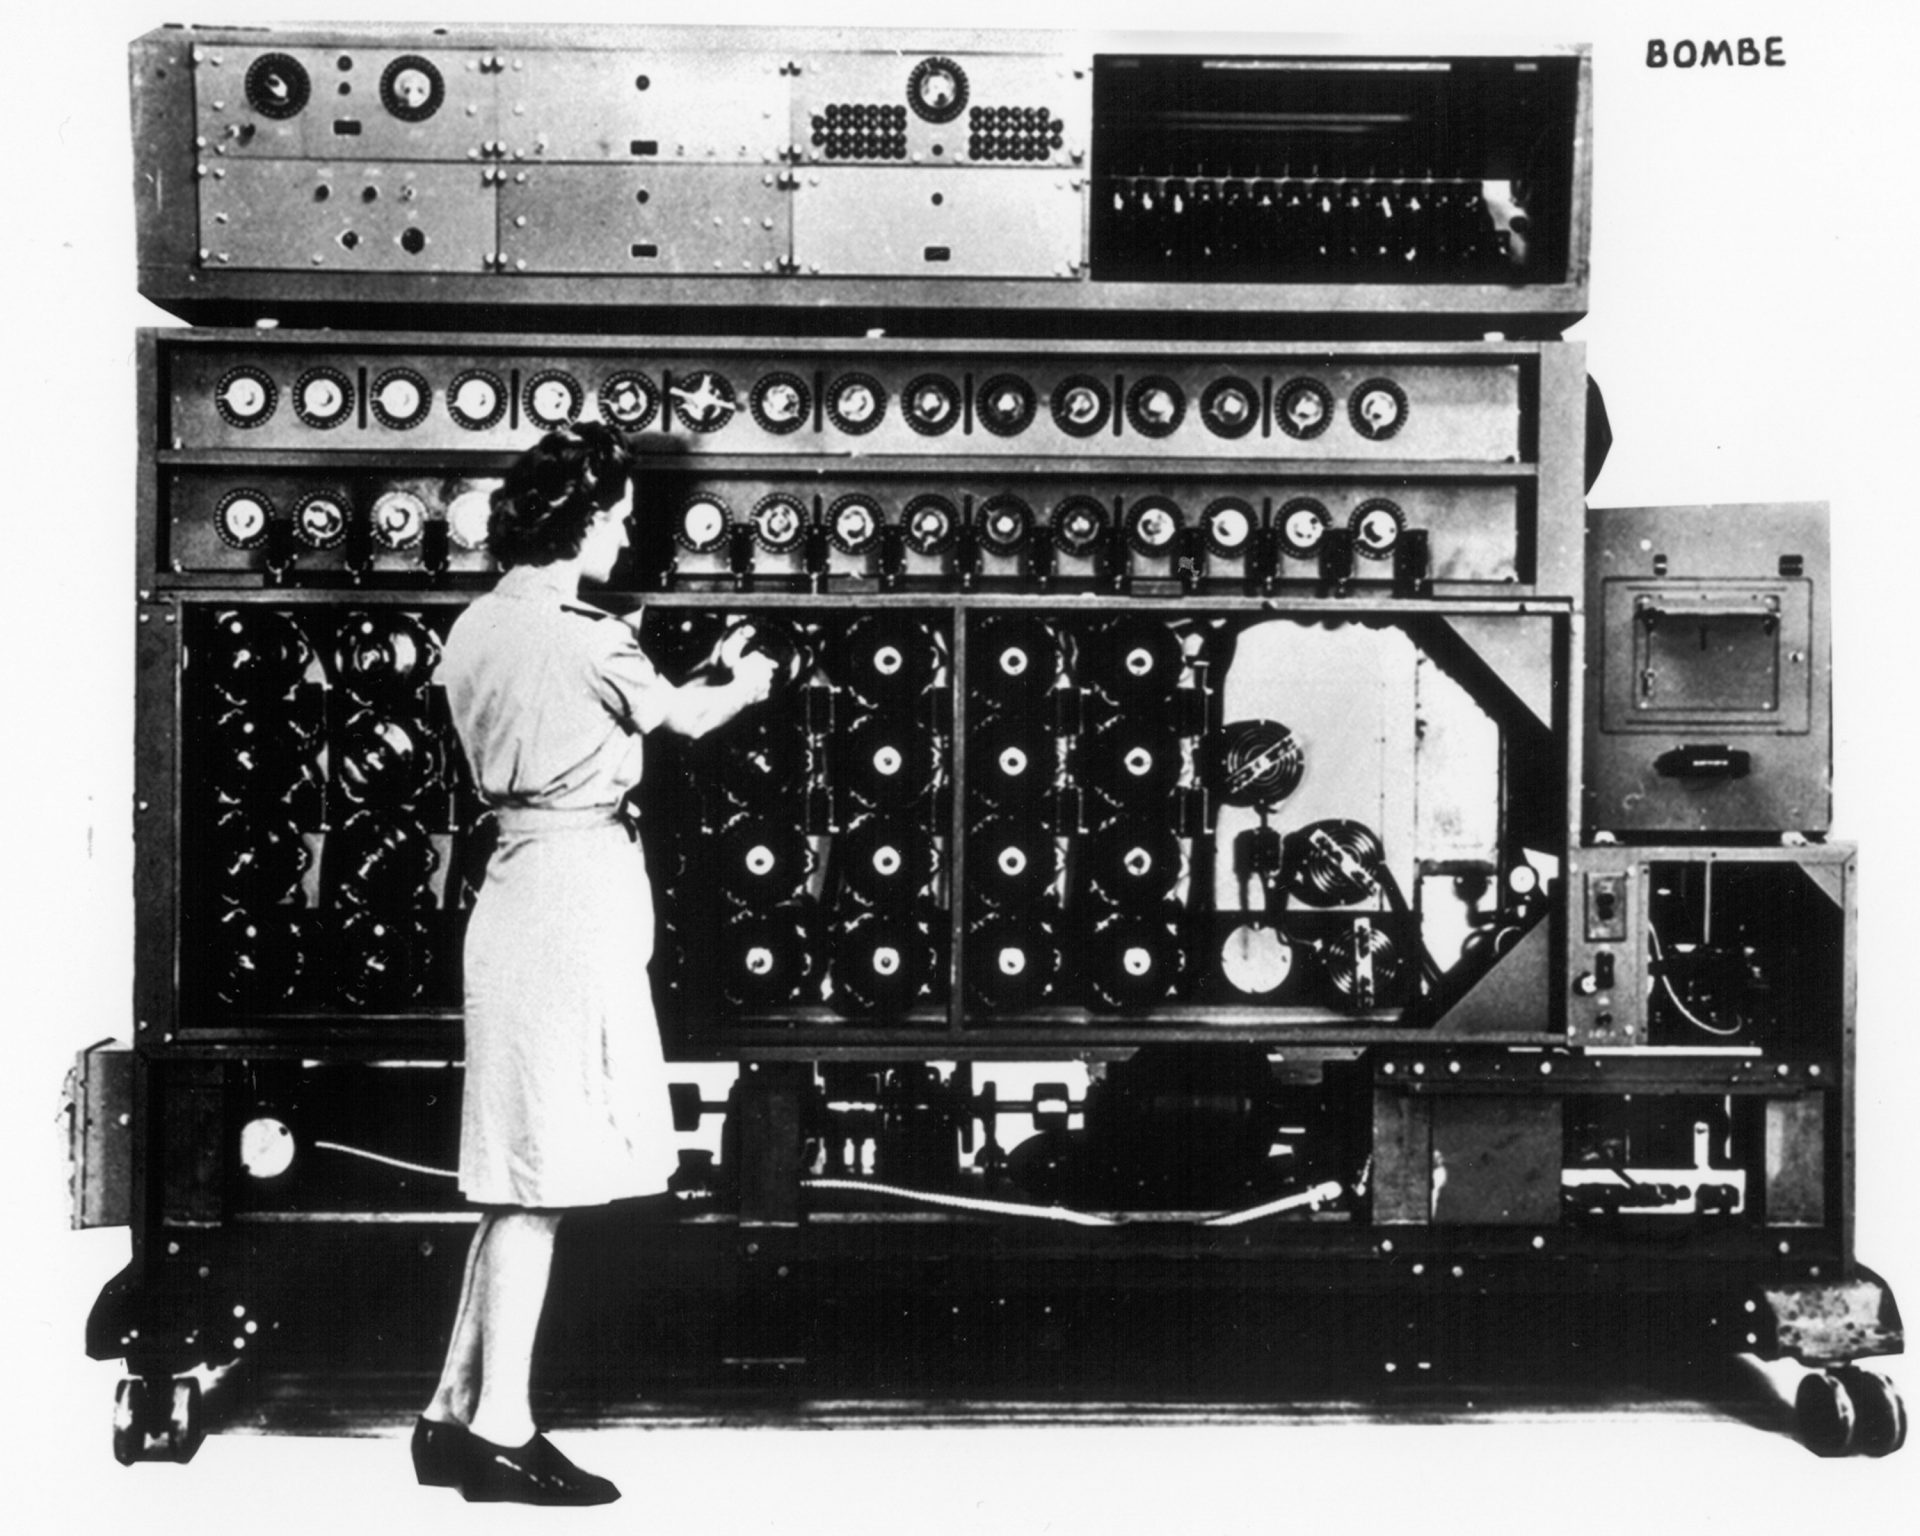
\includegraphics[width=\textwidth]{figs/IMG1}
	\end{minipage}
\end{frame}

\begin{frame}{\textbf{REVOLUTIONIZING INDUSTRIES: THE RISE OF COMPUTERS}}
	\begin{minipage}{0.6\textwidth}
		\textbf{\text In the 1950s and 60s, computers became smaller, faster, and more affordable, leading to their widespread adoption by businesses and governments.}
		\\
		\textbf{\text As a result of the widespread adoption of computers, the number of people in the computing field grew exponentially.}
	\end{minipage}
	\hfill
	\begin{minipage}{0.3\textwidth}
		\centering
		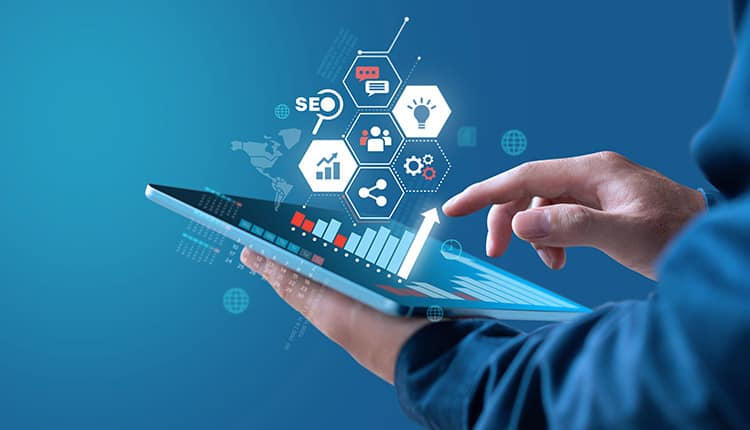
\includegraphics[width=\textwidth]{figs/IMG2}
	\end{minipage}	
\end{frame}

\begin{frame}{\textbf{THE BREAKTHROUGH: APPLE II IN '77}}
	\begin{minipage}{0.6\textwidth}
		\textbf{\text The Apple II, released in 1977, was the first mass-produced personal computer. The Apple II was designed and developed by Steve Wozniak and Steve Jobs in Jobs' family garage.} 
	\end{minipage}
	\hfill
	\begin{minipage}{0.3\textwidth}
		\centering
		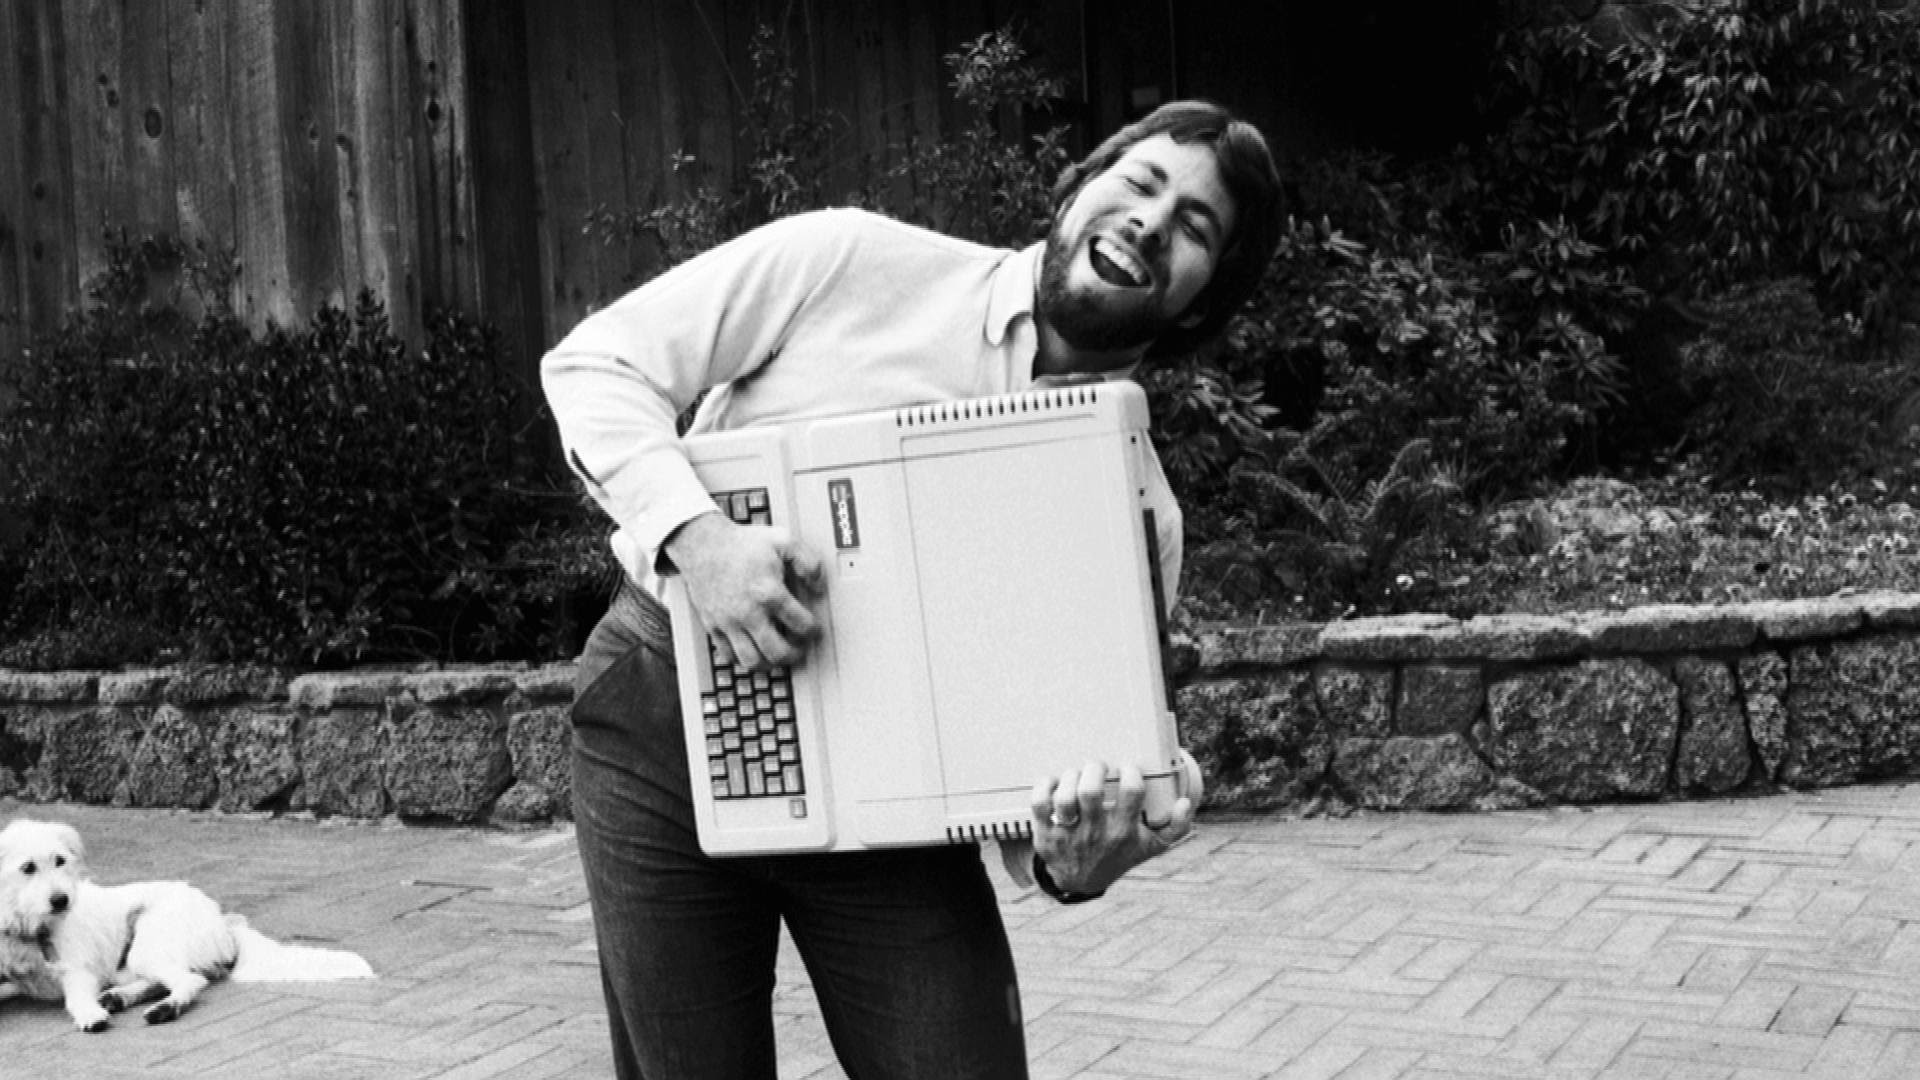
\includegraphics[width=\textwidth]{figs/IMG3}
	\end{minipage}
\end{frame}

\begin{frame}{\textbf{REVOLUTIONIZING PCS: MICROSOFT WINDOWS' GUI INNOVATION}}
	\begin{minipage}{0.6\textwidth}
		\textbf{\text Microsoft Windows, released in 1985, brought GUIs to IBM-compatible PCs. Some of the key features of Windows were its ability to run multiple programs at the same time, and the use of a mouse to navigate and interact with the operating system.} 
	\end{minipage}
	\hfill
	\begin{minipage}{0.3\textwidth}
		\centering
		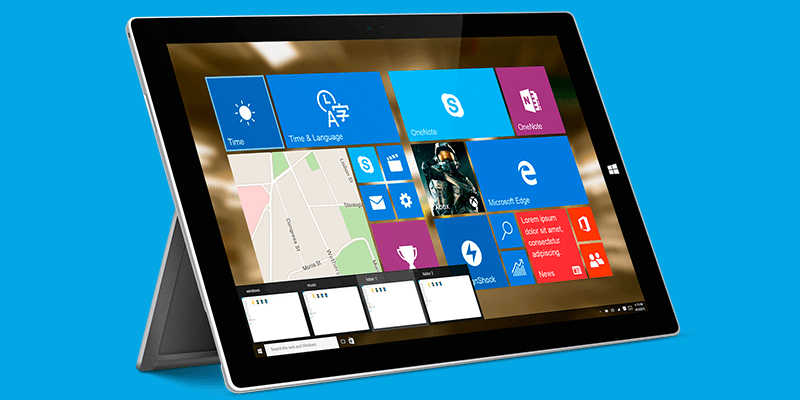
\includegraphics[width=\textwidth]{figs/IMG4}
	\end{minipage}
\end{frame}

\begin{frame}{\textbf{REVOLUTIONIZING CLOUD COMPUTING: AWS 2006}}
	\begin{minipage}{0.6\textwidth}
		\textbf{\text Amazon Web Services (AWS), released in 2006, was one of the first cloud computing platforms.}
		\\
		\textbf{\text Today, AWS is the most comprehensive and widely used cloud service provider with features such as computing, storage, databases, migration, and security.}
	\end{minipage}
	\hfill
	\begin{minipage}{0.3\textwidth}
		\centering
		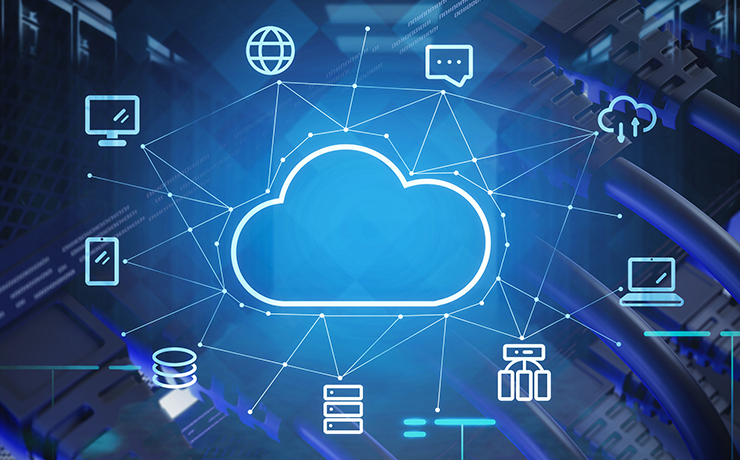
\includegraphics[width=\textwidth]{figs/IMG5}
	\end{minipage}
\end{frame}

\begin{frame}{\textbf{CLOUD COMPUTING: THE NEW NORMAL}}
	\begin{minipage}{0.6\textwidth}
		\textbf{\text Today, cloud computing is ubiquitous, with many companies relying on cloud services for their day-to-day operations. The increased demand for cloud computing has led to the emergence of numerous cloud service providers, each offering unique features and benefits.}
	\end{minipage}
	\hfill
	\begin{minipage}{0.3\textwidth}
		\centering
		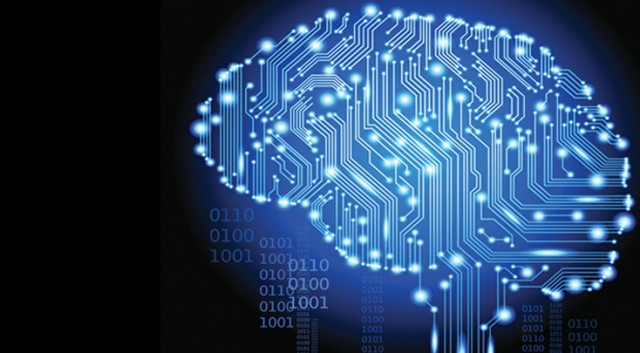
\includegraphics[width=\textwidth]{figs/IMG6}
	\end{minipage}
\end{frame}

\begin{frame}{\textbf{REVOLUTIONARY TECH ACROSS INDUSTRIES}}
	\begin{minipage}{0.6\textwidth}
		\textbf{\text These technologies are being used in a variety of industries, from healthcare to finance to transportation. In healthcare, technologies such as telemedicine and wearable devices have been transformative, allowing doctors to remotely monitor and diagnose patients.}
	\end{minipage}
	\hfill
	\begin{minipage}{0.3\textwidth}
		\centering
		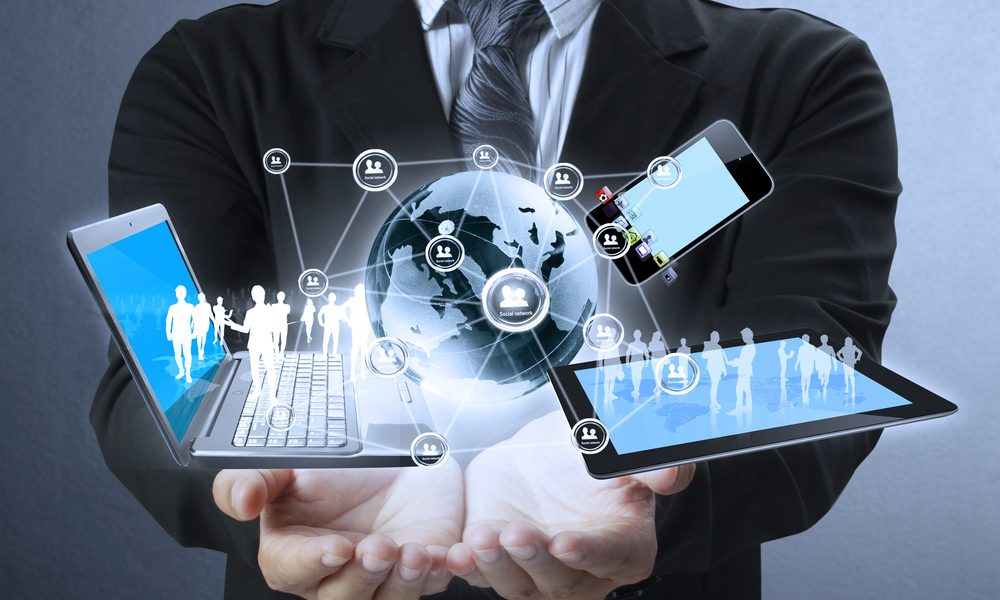
\includegraphics[width=\textwidth]{figs/IMG7}
	\end{minipage}
\end{frame}

\begin{frame}{\textbf{QUANTUM COMPUTING: SOLVING THE IMPOSSIBLE}}
	\begin{minipage}{0.6\textwidth}
		\textbf{\text These computers have the potential to solve problems that are currently impossible to solve with classical computers. Quantum computers use qubits instead of bits, which allow for exponential increases in computing power.}
	\end{minipage}
	\hfill
	\begin{minipage}{0.3\textwidth}
		\centering
		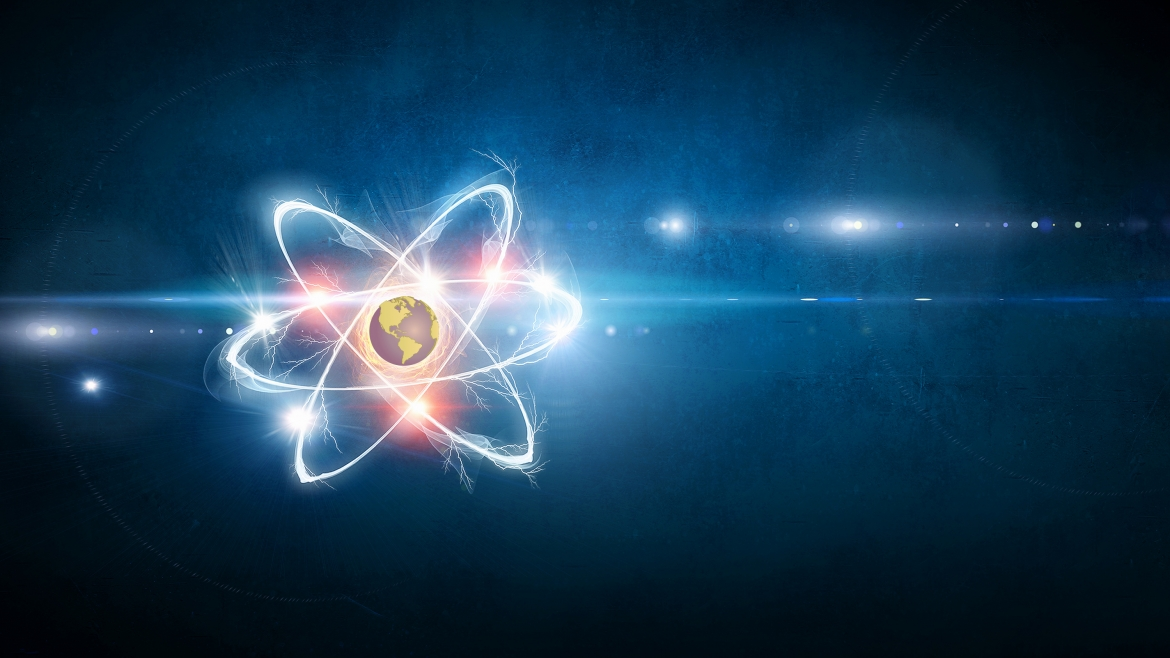
\includegraphics[width=\textwidth]{figs/IMG8}
	\end{minipage}
\end{frame}

\begin{frame}{\textbf{THE FUTURE OF COMPUTING: UNCERTAIN BUT CRUCIAL}}
	\begin{minipage}{0.6\textwidth}
		\textbf{\text It is impossible to predict exactly what the future of computing holds, but it is clear that computing will continue to play a critical role in our lives. Whether it's through artificial intelligence, quantum computing, or advancements in software and hardware engineering, the speed and capabilities of the computers we use will continue to increase.}
	\end{minipage}
	\hfill
	\begin{minipage}{0.3\textwidth}
		\centering
		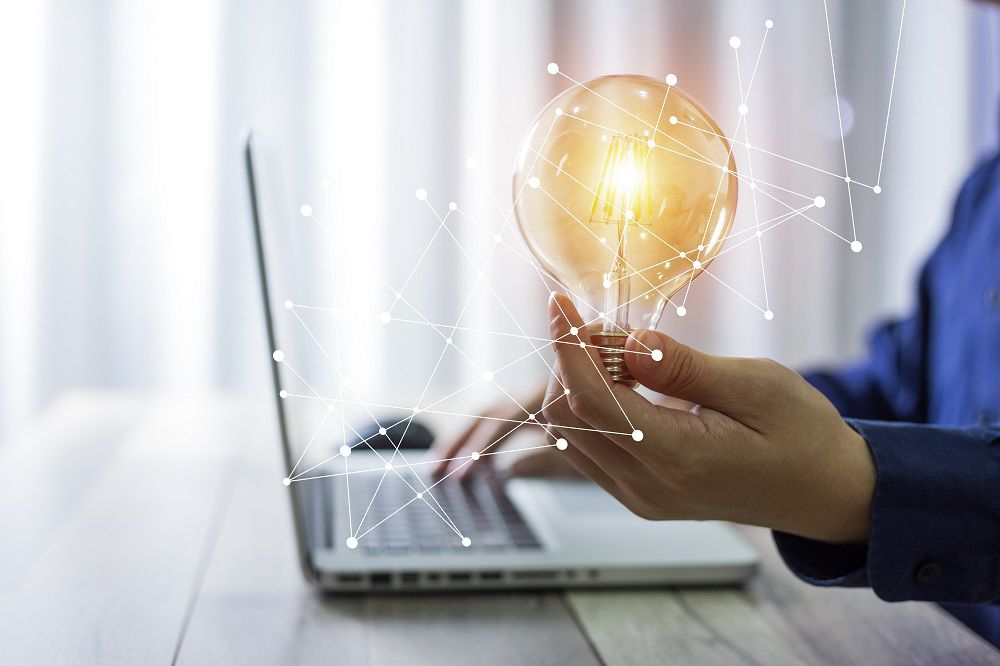
\includegraphics[width=\textwidth]{figs/IMG9}
	\end{minipage}
\end{frame}

\begin{frame}{\textbf{BEYOND THE SCREEN: COMPUTING'S FUTURE INNOVATIONS}}
	\begin{minipage}{0.6\textwidth}
		\textbf{\text In conclusion, the evolution of computing has been a fascinating journey, from the mechanical calculators of the 1800s to the powerful cloud computing platforms of today.}
		\\
		\textbf{\text Computing has transformed the way we live, work, and communicate, and will continue to do so in the future.}
	\end{minipage}
	\hfill
	\begin{minipage}{0.3\textwidth}
		\centering
		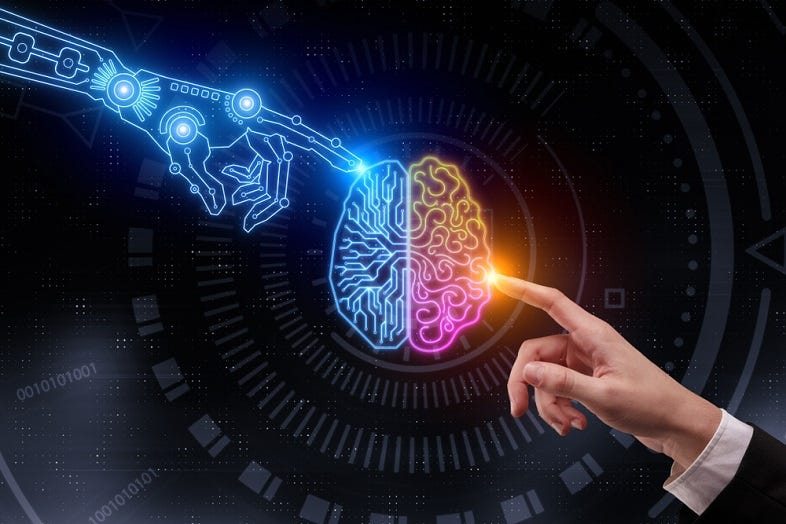
\includegraphics[width=\textwidth]{figs/IMG10}
	\end{minipage}
\end{frame}
\end{document}
